\section{Corpus and Protocol}
\label{sec:method}

\subsection{Corpus}
The corpus is constructed from three CVE-anchored sources: BigVul, CVEfixes, and Devign. Each sample represents an actual function extracted from a real project. Functions are transformed into Code Property Graphs using Joern 4.0 and exported in the \texttt{cpg14} per-method format. Table~\ref{tab:corpus} gives the composition.

\begin{table}[h]
\centering
\caption{Corpus composition.}
\label{tab:corpus}
\begin{tabular}{lrr}
\toprule
& \textbf{Graphs} & \textbf{Vulnerable} \\
\midrule
BigVul (vulnerable)      & 10,763 & 10,763 \\
BigVul (re-sampled safe) & 78,510 & 0 \\
CVEfixes (paired)        & 15,346 & 7,673 \\
Devign                   & 27,284 & 12,445 \\
\midrule
\textbf{Total}           & \textbf{131,903} & \textbf{30,881} \\
\multicolumn{3}{l}{949 repositories, 17,968 commits, 23.4\% prevalence} \\
\bottomrule
\end{tabular}
\end{table}


\subsection{Split protocols}
\label{sec:protocols}
All protocols partition the same corpus, differing only in the extent to which the test partition may overlap with the training partition. Figure~\ref{fig:split} shows what each permits to cross.

\begin{description}[leftmargin=1.2em,itemsep=2pt]
  \item[\texttt{random}] A stratified shuffle over individual functions. This is the protocol used by most published work, and it is included as an experimental control, not as a way to report a better number.
  \item[\texttt{group}] Pair-, commit- and clone-family-grouped, repositories still shared. Isolates what repository overlap alone is worth.
  \item[\texttt{repo}] Repository-disjoint: no project appears in more than one partition.
\end{description}

\subsubsection{Near-duplicate detection}
Exact and near-duplicate functions are collapsed into clone families before splitting, and a family is atomic, following the recommendation that duplicate code be separated across partitions in models of code~\citep{allamanis2019adverse}. Detection is a MinHash~\citep{broder1997resemblance} over token 5-shingles of each CPG's node code attributes. Banding produces candidates only; every candidate pair is verified against the full signature before being unioned, because unioning candidates directly allows single-linkage chaining. In one run this collapsed the entire corpus into a single family. We validated the estimator against true Jaccard on 240 sampled pairs: it is essentially unbiased (mean signed error $+0.002$) with mean absolute error $0.017$. Halving to $N_{\text{perm}}=64$ raises that error to $0.024$, and because a false negative is the costly direction for a leakage control we use $128$.

\begin{figure}[htb]
\centering
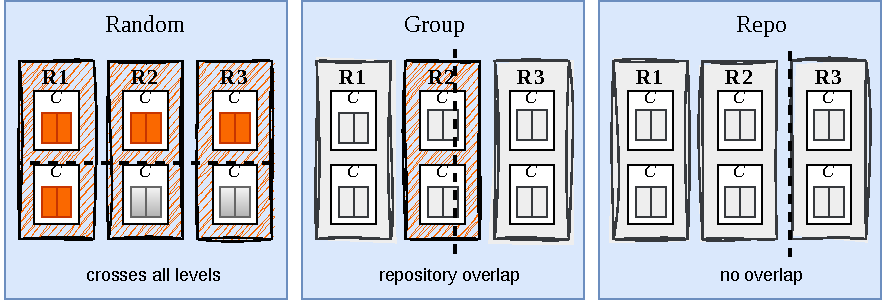
\includegraphics[width=\textwidth]{split.pdf}
\caption{What each protocol permits to cross the train/test boundary. Three
repositories (R1--R3), each holding commits (C), each holding a vulnerable
function and its patched counterpart. Hatching marks material appearing on both
sides of the split. All three protocols partition the identical corpus; only
the level at which the cut is made changes.}
\label{fig:split}
\end{figure}

\subsubsection{Audited disjointness}
Every split ships an audit over four keys. Table~\ref{tab:audit} reports them;
the \texttt{random} row is what a plain stratified shuffle admits.

\begin{table}[h]
\centering
\caption{Train/test overlap by key. The \texttt{random} row is the control.}
\label{tab:audit}
\begin{tabular}{lrrrr}
\toprule
\textbf{Protocol} & \textbf{repo} & \textbf{commit} & \textbf{pair} & \textbf{clone} \\
\midrule
\texttt{repo}   & 0 & 0 & 0 & 0 \\
\texttt{group}  & 197\rlap{$^\dagger$} & 0 & 0 & 0 \\
\texttt{random} & 626 & 3,717 & 1,590 & 3,186\rlap{$^\ddagger$} \\
\bottomrule
\end{tabular}
\begin{tablenotes}\footnotesize
\item $^\dagger$ By design: \texttt{group} does not separate repositories.
\item $^\ddagger$ \texttt{random} is built without clone-family atomicity, since
it is the control, so its clone overlap is measured after the fact rather than
enforced. 3,771 test functions belong to a family that also appears in training.
\item Under \texttt{random}, 1,590 functions appear in training alongside their
own patched counterpart in test: the same function, differing by the fix, with
the opposite label.
\end{tablenotes}
\end{table}


\subsection{Models and controls}
All model backbones use identical node features (GraphCodeBERT embeddings of each node's code, concatenated with a learned node-type embedding), as well as identical pooling, loss function, optimizer, folds, and metrics. Only the specified component varies. Each node is described by two concatenated vectors: a 768-dimensional GraphCodeBERT~\citep{guo2021graphcodebertpretrainingcoderepresentations} embedding of its code, truncated at 128 tokens, and a 64-dimensional learned embedding of its syntactic type. Each edge carries a 32-dimensional learned embedding of its relation type.

\begin{description}[leftmargin=1.2em,itemsep=2pt]
  \item[Architectures] Graph Attention Network (GAT)~\citep{DBLP:conf/iclr/VelickovicCCRLB18}, Graph Convolutional Network (GCN)~\citep{Kipf2016SemiSupervisedCW}, Graph Isomorphism Network (GIN)~\citep{xu2018how} and a Graph Transformer~\citep{3454287.3455360,shi2021masked}, spanning attention, spectral convolution, sum aggregation and global attention. All are the reference implementations in PyTorch Geometric~\citep{fey2019fast}; the typed-edge condition uses its relational convolution~\citep{schlichtkrull2018modeling} where the operator has no edge-feature term.
  \item[\texttt{no graph}] Every edge deleted; depth, width and pooling unchanged. Isolates structure from text.
  \item[\texttt{untyped}] All four CPG relation types (AST, CFG, DDG, CDG) collapsed to one. Isolates edge-type information.
  \item[\texttt{type-only}] Node text zeroed; the model sees the graph and each node's syntactic kind but never an identifier or literal.
  \item[\texttt{topology}] Text zeroed and node types collapsed. Nothing survives but graph shape. This is the floor, and it is what makes a non-zero \texttt{type-only} result interpretable, since graph size alone correlates with the label.
  \item[bag-of-words] Node features replaced with hashed token counts at identical width. A weak-encoder control for the objection that strong features leave the graph nothing to add.
\end{description}


\subsection{Metrics}
ROC-AUC is reported as the primary metric because it is invariant to prevalence, which varies across protocols. Since macro-F1 alone is insufficient for evaluating a detector at a realistic base rate, PR-AUC, MCC, false-positive rate, and recall at fixed false-positive budgets are also reported, each referenced against its partition's prevalence.

\subsection{Reporting variance}
\label{sec:variance}
Run-to-run standard deviation on this task is approximately $0.010$, which is comparable to the magnitude of several measured effects. Principal results are reported over five seeds when the claim depends on a small difference, and over three seeds otherwise, with the count specified, and differences are tested rather than read off the means~\citep{arcuri2011practical}. Each run also records per-fold test scores. Section~\ref{sec:variance-result} demonstrates the importance of this approach: every single-seed estimate reported there disagrees with its five-seed mean, one of them by a factor of twenty-eight, and individual seeds disagree with the mean in sign in all three cases.
